\documentclass[9pt]{article}

\usepackage{graphicx}
\usepackage{epstopdf}
\usepackage{float}

\begin{document} 



\begin{titlepage}
\title{\textbf{Capstone Proposal: Style Transfer}}
\author{Ravi Rai}
\maketitle

\end{titlepage}

\newpage
\section{Domain Background}
In the subject of Machine Learning, there is an artistic problem called Style Transfer. Style Transfer lies in the field of deep neural networks and image classification, and while it is a relatively new problem, it has already seen a few notable solutions. One such solution is in Gatys' paper \cite{Neural}, in which this project will follow quite closely. Image classification is a popular problem in machine learning, where the goal is to detect specific objects in any given image, and it has many applications like face detection and even self-driving cars. The methodology of image classification is to use neural networks, which essentially have small image filters that try and detect import features in images, and associate them with an object of interest. A collection of these image filters can provide necessary texture information, which we can call the style of an image. In the past, capturing the style of an image was used to detect the time periods of other images (by seeing if they had a similar style), but the idea of Style Transfer is to capture the style of some image, and recreate another image with that same style. This problem could be done by artists on their own, but the problem was that there was no real way to formulate or replicate Style Transfer results. However, with the help of image classification, interest in solving this problem with Machine Learning developed, and there are now replicable results.

\section{Problem Statement}
The problem in this project is to replicate Figure 2C in \cite{Neural} as closely as possible. The image Figure 2C in \cite{Neural} can be used as a guidance for how well my solution works, and is essentially the solution to the project. There will also be a loss function by which accuracy can be measured. This loss function is a combination of both the style loss and content loss. Here, the content loss refers to the content image, which is the basis image that we are trying to recreate with a different style. The content loss is essentially a difference between the features on the original/content image and the  image that the neural network will create. Similarly, the style loss refers to the image whose style we are trying to capture. The style loss function will also be made up of a difference between the original style image and the image that the neural network creates. The total loss function will be a combination of both of these two style functions, and will be of the form:
\begin{equation}
Loss_{total} = \alpha * Loss_{content} + \beta * Loss_{style}
\end{equation}
$\alpha$ and $\beta$ will be tuned by trail and error to give the most optimal results. The ultimate solution will be to replicate figure 2C in \cite{Image}, while simultaneously minimizing the loss function such that the result is reproducible.

\begin{figure}
\centering
        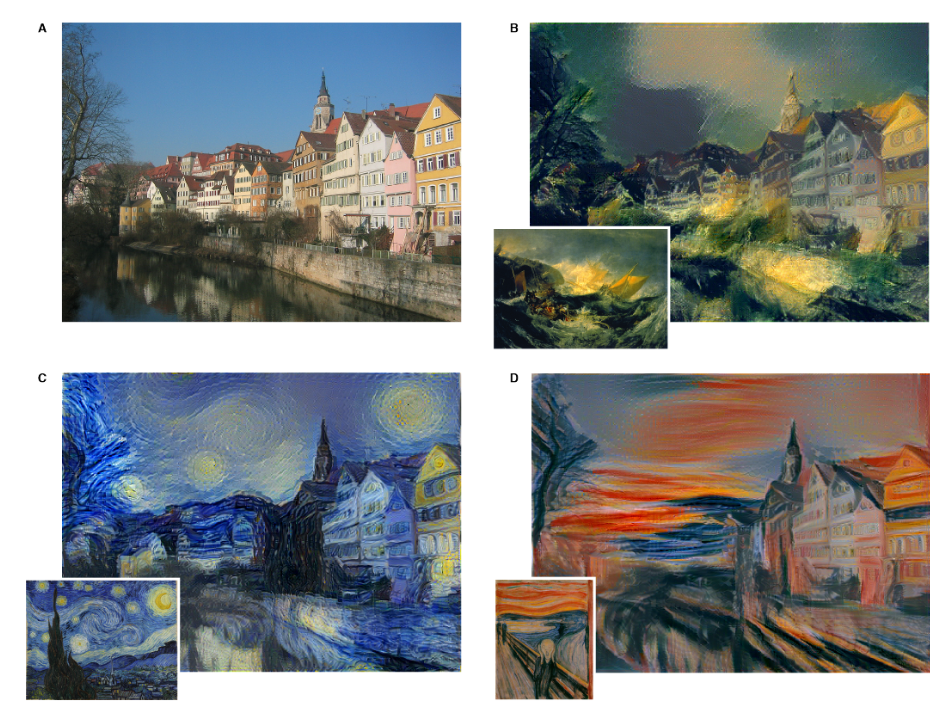
\includegraphics[totalheight=8cm]{Figure2.png}
    \caption{Figure 2 (A-D) used in \cite{Neural}. Image C is the solution image, with the image on the bottom left being the style image, and image A being the content image. Figure 2 in \cite{Neural} is identical to Figure 3 in \cite{Image}}
    \label{fig:solution}
\end{figure}

\section{Datasets and Inputs}
The inputs would be the content image (Figure 2A in \cite{Neural} or Figure 1A from above image) and ``The Starry Night" by Vincent van Gogh, 1889 (bottom left image of Figure C from above). Any two images could be used for this project, however; in the interest of having a reference solution, I chose these so that I can easily compare my projects output to Figure 2C in \cite{Image}. I will get the images from Google images. I will fix the height and width of the images so that they are the same (the dimension of the content image is 450x345, and 1024x786 for the style image, so the image sizes will be fixed to 450x345, since stratching images to a larger size may cause unneccessary blurryness). Fixing the image size will help prevent any discrepancies in the output, and was done in \cite{Neural}. Also, there will be a white noise image involved in this project (explained later), and this will also have dimension 450x345. The inputs for this project will just be these two images (and some white noise image), which will contain pixel information which would be the dataset. The model of this project should work given just one content image and one style image (using a pre-trained network).

Some important noticeable qualities of the content image are that it is a sequence of connected houses, with a church-like building sticking out in the background. Also, these houses are right next to a body of water, with a tree sticking out on the left side of the image. Theses details of the content image are important to note because they are fundamental details, and should be expected to appear clearly in the output image. The style image (Starry Night), has some important details as well, although since it is the style of the image that matters, the objects in the image are not necessarily the fundamental details. Rather, some important details to note about this style image - that might appear in the output image - are the circular motions in the image, the different shades of blue crayon-like colouring, along with the yellow spots. Also, the dark green tree-like object on the left side of the image is an important feature because of the different color appearing on the left side only (the fact that it looks like a separate object does not matter so much, since the style of the image is of more concern than the objects themselves). 


\section{Solution Statement}
The solution to the problem will be Figure 2C in \cite{Neural} or Figure 3C in \cite{Image}. The goal is to create an image the looks as much as the solution image as possible, which will involve minimizing the loss function above. Also, it is expected that the higher $\alpha$ is, the more clear the content image is in the output image, and the higher $\beta$ is, the more stylistic the output image is. This can be checked by comparing an $\alpha/\beta$ ratio, and a similar output as Figure 4 in \cite{Image} will show this. Ultimately, the solution is to get an output image that consistently can reproduce similar results as in \cite{Neural, Image}. The solution will be measured by the loss function, which should be a reoccurring value. In regards to recreating Figure 2C in \cite{Neural} (or Figure 3C in \cite{Image}), the $\alpha/\beta$ ratio should be similar to \cite{Image}, which is $8 \times 10^{-4}$.

\begin{figure}[H]
\centering
        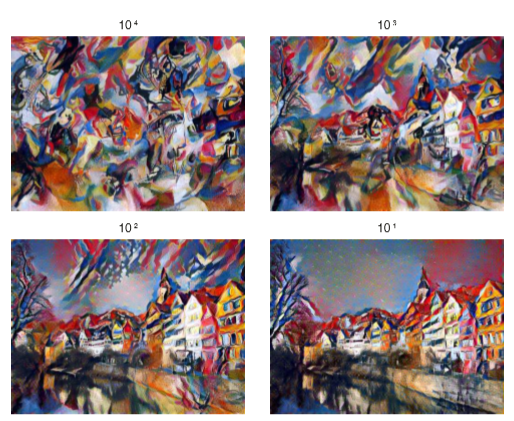
\includegraphics[totalheight=8cm]{Figure4AlphaBetaRatios.png}
    \caption{Figure 4 from \cite{Image}, showing how the $alpha$ and $beta$ values can affect the output image (although with a different style image than this project). The numbers at the top are $\alpha/\beta$ ratios.}
    \label{fig:solution}
\end{figure}

\section{Benchmark Model}
The benchmark model follows from the model in the methods section of \cite{Neural} and from section 2 of \cite{Image}. The idea is to use a pre-trained image classification network, like VGG19, to get feature maps of both the style and content images. There will be a base input image, which will be white noise, and it will have its own feature map. The content loss function ($Loss_{content}$) will be obtained by taking the squared difference of the content image feature map and the input image feature map at each layer of the network, and then summing them up. 

Obtaining a representation of the style image is slightly different, where now texture information is sought after. Gram matrices represent feature correlations between different filter responses in the neural network, and they will give the desired texture information, and nothing more. Using a function to compute Gram matrices in each layer of a neural network, one can then - as before - calculate the squared difference between the Gram matrices of the input image and style image, and this essentially makes up the loss function for the style image ($Loss_{style}$). Finally, to get the desired output image with the content of the content image and style of the style image, we must simultaneously minimize both loss functions. This loss function is measurable, and it is how the model will be ultimately be evaluated.

\section{Evaluation Metrics}
The performance of the model can be measured by the total loss function ($Loss_{total}$) from above, and by the output image. If the output image is obviously not similar to the intended solution image in \cite{Neural, Image}, but the total loss function is minimal, then one would rate the model as a failing model. Similarly, if the output image is clearly similar to the solution image, but the total loss function outputs a large value, then one should rate the model as a failing model as well. These are extreme cases, and more likely if the loss function is minimal, the output image will look similar to the intended solution (and vice versa). Because of this, when evaluating the model, one should check that neither extreme cases are occurring, and then can proceed by evaluating the model based on the total loss function. One evaluation would be to run the model multiple times, and evaluate the model by dividing the best loss function by the worst out of all the iterations. So if the loss function outputted a $10^8$ in one of the iterations, and another (worse) iteration outputted a loss function value of $10^{10}$, then the model would get a 1 percent.

\section{Project Design}
To create a model that can take two images and recreate one with the style of another (should work for any two images), the first step is to handle the input data first. Here the input data are just images, and the only thing that needs to be done to them is that they must be fixed to the same size. For the purpose of this project, fixing the chosen images to be the same size is all that needs to be done, so whichever image is larger can be resized to match the size of the smaller image. A white noise image will also be used, which will also be fixed to be the same size. 

Next, a pre-trained image classifier will be used to get the content and style representations of the images. Different networks can be attempted and used to see what gives the best result, but the VGG19 network was used in \cite{Neural, Image}, so this will be used if there is no time to try the others. To set up the loss function, the first step is to get the content loss function. As explained above, to get the content loss function, intermediate layer feature maps will be used iteratively to get the difference between these feature maps and the white noise feature maps, and then they will be squared and summed up. The style loss function will be obtained the same way except by using Gram matrices instead of feature maps. The intermediate layers used will be the same ones as in \cite{Neural}. Finally, the loss function will be a linear combination of the two different loss function, with coefficients that can be changed to get optimal results (some coefficient ratios are given in \cite{Neural, Image}). 

The Final step will be to use gradient decent to minimize the loss function. Their are other ways to minimize the loss function, which could also be explored to get better results, or perhaps similar results but in less time (like the Adam optimizer). \cite{Neural} describes what the gradient of the content and style loss functions look like, and that standard error back-propagation can be used to calculate the gradient. Since the loss function is a linear combination, both loss functions will be minimized at the same time, so the weights $\alpha$ and $\beta$ from the above equation will play an important role in getting the best model. \cite{Neural} gives an $\alpha/\beta$ ratio to try, and from there the best $\alpha/\beta$ ratio will be found by use of trial and error. Finally, using the loss functions, a model, which can be a function itself (given content and style images as inputs), will be made to return the output image (which would be a transformed white noise image).

\newpage

\bibliographystyle{unsrt}
\addcontentsline{toc}{section}{Bibliography}
\bibliography{Bibliographyproposal}

\end{document}


